%%%%%%%%%%%%%%%%%%%%%%%%%%%%%%%%%%%%%%%%%%%%%%%%%%%%%%%%%%%%%%%%%%%%%%%%%%%%
%% Author template for INFORMS Journal on Computing (ijoc)
%% Mirko Janc, Ph.D., INFORMS, mirko.janc@informs.org
%% ver. 0.95, December 2010
%%%%%%%%%%%%%%%%%%%%%%%%%%%%%%%%%%%%%%%%%%%%%%%%%%%%%%%%%%%%%%%%%%%%%%%%%%%%
%\documentclass[ijoc,blindrev]{informs3}
\documentclass[ijoc,nonblindrev]{informs3} % current default for manuscript submission

%%\OneAndAHalfSpacedXI
\OneAndAHalfSpacedXII % current default line spacing
%%\DoubleSpacedXII
%%\DoubleSpacedXI

% If hyperref is used, dvi-to-ps driver of choice must be declared as
%   an additional option to the \documentclass. For example
%\documentclass[dvips,ijoc]{informs3}      % if dvips is used
%\documentclass[dvipsone,ijoc]{informs3}   % if dvipsone is used, etc.

% Private macros here (check that there is no clash with the style)

% Natbib setup for author-year style
\usepackage{natbib}
 \bibpunct[, ]{(}{)}{,}{a}{}{,}%
 \def\bibfont{\small}%
 \def\bibsep{\smallskipamount}%
 \def\bibhang{24pt}%
 \def\newblock{\ }%
 \def\BIBand{and}%

%% Setup of theorem styles. Outcomment only one.
%% Preferred default is the first option.
\TheoremsNumberedThrough     % Preferred (Theorem 1, Lemma 1, Theorem 2)
%\TheoremsNumberedByChapter  % (Theorem 1.1, Lema 1.1, Theorem 1.2)

%% Setup of the equation numbering system. Outcomment only one.
%% Preferred default is the first option.
\EquationsNumberedThrough    % Default: (1), (2), ...
%\EquationsNumberedBySection % (1.1), (1.2), ...

% In the reviewing and copyediting stage enter the manuscript number.
%\MANUSCRIPTNO{} % When the article is logged in and DOI assigned to it,
                 %   this manuscript number is no longer necessary

%%%%%%%%%%%%%%%%
\begin{document}
%%%%%%%%%%%%%%%%

% Outcomment only when entries are known. Otherwise leave as is and
%   default values will be used.
%\setcounter{page}{1}
%\VOLUME{00}%
%\NO{0}%
%\MONTH{Xxxxx}% (month or a similar seasonal id)
%\YEAR{0000}% e.g., 2005
%\FIRSTPAGE{000}%
%\LASTPAGE{000}%
%\SHORTYEAR{00}% shortened year (two-digit)
%\ISSUE{0000} %
%\LONGFIRSTPAGE{0001} %
%\DOI{10.1287/xxxx.0000.0000}%

% Author's names for the running heads
% Sample depending on the number of authors;
% \RUNAUTHOR{Jones}
% \RUNAUTHOR{Jones and Wilson}
% \RUNAUTHOR{Jones, Miller, and Wilson}
% \RUNAUTHOR{Jones et al.} % for four or more authors
% Enter authors following the given pattern:
%\RUNAUTHOR{}

% Title or shortened title suitable for running heads. Sample:
% \RUNTITLE{Bundling Information Goods of Decreasing Value}
% Enter the (shortened) title:
%\RUNTITLE{}

% Full title. Sample:
% \TITLE{Bundling Information Goods of Decreasing Value}
% Enter the full title:
%\TITLE{}

% Block of authors and their affiliations starts here:
% NOTE: Authors with same affiliation, if the order of authors allows,
%   should be entered in ONE field, separated by a comma.
%   \EMAIL field can be repeated if more than one author
\ARTICLEAUTHORS{%
\AUTHOR{Susann Goldstein}
\AFF{\EMAIL{goldstein.susann@gmail.com}}
\AUTHOR{Diana Hornig}
\AFF{\EMAIL{Hornig.Diana@gmail.com}}
\AUTHOR{Olena Vyshnevska}
\AFF{\EMAIL{olenavshn@gmail.com}}
\AUTHOR{Simon Bordewisch}
\AFF{\EMAIL{bordewisch@studserv.uni-leipzig.de}}
\AUTHOR{Dennis Kreußel}
\AFF{\EMAIL{dennis.kreussel94@gmail.com}}

% Enter all authors
} % end of the block

\ABSTRACT{%
Text of your abstract % Enter your abstract
}%

% Sample
%\KEYWORDS{deterministic inventory theory; infinite linear programming duality;
%  existence of optimal policies; semi-Markov decision process; cyclic schedule}

% Fill in data. If unknown, outcomment the field
\KEYWORDS{}
\HISTORY{}

\maketitle
%%%%%%%%%%%%%%%%%%%%%%%%%%%%%%%%%%%%%%%%%%%%%%%%%%%%%%%%%%%%%%%%%%%%%%

% Samples of sectioning (and labeling) in IJOC
% NOTE: (1) \section and \subsection do NOT end with a period
%       (2) \subsubsection and lower need end punctuation
%       (3) capitalization is as shown (title style).
%
%\section{Introduction.}\label{intro} %%1.
%\subsection{Duality and the Classical EOQ Problem.}\label{class-EOQ} %% 1.1.
%\subsection{Outline.}\label{outline1} %% 1.2.
%\subsubsection{Cyclic Schedules for the General Deterministic SMDP.}
%  \label{cyclic-schedules} %% 1.2.1
%\section{Problem Description.}\label{problemdescription} %% 2.

% Text of your paper here

Lorem ipsum dolor sit amet, consectetur adipisicing elit, sed do eiusmod
tempor incididunt ut labore et dolore magna aliqua. Ut enim ad minim
veniam, quis nostrud exercitation ullamco laboris nisi ut aliquip ex ea
commodo consequat. Duis aute irure dolor in reprehenderit in voluptate
velit esse cillum dolore eu fugiat nulla pariatur. Excepteur sint
occaecat cupidatat non proident, sunt in culpa qui officia deserunt
mollit anim id est laborum.

Sed ut perspiciatis unde omnis iste natus error sit voluptatem
accusantium doloremque laudantium, totam rem aperiam, eaque ipsa quae ab
illo inventore veritatis et quasi architecto beatae vitae dicta sunt
explicabo. Nemo enim ipsam voluptatem quia voluptas sit aspernatur aut
odit aut fugit, sed quia consequuntur magni dolores eos qui ratione
voluptatem sequi nesciunt. Neque porro quisquam est, qui dolorem ipsum
quia dolor sit amet, consectetur, adipisci velit, sed quia non numquam
eius modi tempora incidunt ut labore et dolore magnam aliquam quaerat
voluptatem. Ut enim ad minima veniam, quis nostrum exercitationem ullam
corporis suscipit laboriosam, nisi ut aliquid ex ea commodi consequatur?
Quis autem vel eum iure reprehenderit qui in ea voluptate velit esse
quam nihil molestiae consequatur, vel illum qui dolorem eum fugiat quo
voluptas nulla pariatur?

At vero eos et accusamus et iusto odio dignissimos ducimus qui
blanditiis praesentium voluptatum deleniti atque corrupti quos dolores
et quas molestias excepturi sint occaecati cupiditate non provident,
similique sunt in culpa qui officia deserunt mollitia animi, id est
laborum et dolorum fuga. Et harum quidem rerum facilis est et expedita
distinctio. Nam libero tempore, cum soluta nobis est eligendi optio
cumque nihil impedit quo minus id quod maxime placeat facere possimus,
omnis voluptas assumenda est, omnis dolor repellendus. Temporibus autem
quibusdam et aut officiis debitis aut rerum necessitatibus saepe eveniet
ut et voluptates repudiandae sint et molestiae non recusandae. Itaque
earum rerum hic tenetur a sapiente delectus, ut aut reiciendis
voluptatibus maiores alias consequatur aut perferendis doloribus
asperiores repellat.

\input{1_introduction}
\section{Background}
% why you thought the project was needed / your interest in the project
\input{aims}

% technical/social/backgrounds
\subsection{Technical Background}
% ================== !!!!! ======================
% small text here describing which api's we used
% ================== !!!!! ======================
%\input{gtd}         % Dennis
%\subsubsection{Guardian API}
\label{sec:guardian-api}

As our source of global news we have chosen a British newspaper \textit{The Guardian}. Its open platform provides access to over 1.9 billion pieces of content while its \textit{Explore} tool makes it easy to search through the data. We encountered no problems requesting a developer API-key, nor were there any difficulties accessing the data. 

\textit{The Guardian} allows to extract up to 200 articles at a time, however either there is no upper limit on the number of requests one can send using one API-key or the limit is above the scope of our project.

Furthermore, one could also add such filters as "from-date", "to-date", "page size", "order-by" etc. to customise the search. We have used the date-related filters to exclude the content pieces before 2000 and after 2016 as well as increased the "page size" to the maximum of 200 items. 

Having applied the above mentioned filters, we have proceeded with extracting meta-data about ca. 40000 articles with the keyword "terror". Although OpenRefine is an easy tool to clean unsorted meta data, it proved to be inefficient in accessing over 200 URLs of data. Therefore we opted for writing scripts in Python, which would allow us to iterate over all articles without manually specifying the URL of every page. 

The script for extracting meta data from \textit{The Guardian} is similar to the one for \textit{Die Zeit}. The parameters and the keywords were adjusted, the number of items per page was set as well as only meta data was collected, without accessing individual articles. Unfortunately, the articles did not contain information on the location associated with the content piece, neither did they contain tags. 

The results of running the Python script were written into a .csv file and visualised with plot.ly.

\begin{figure}[h]
  \centering
  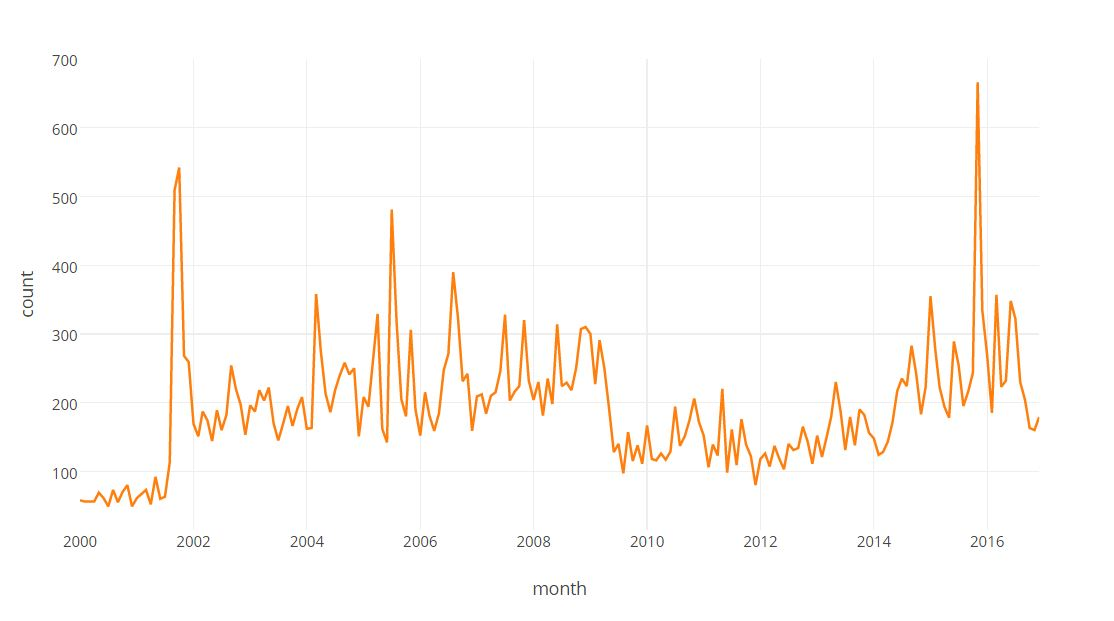
\includegraphics[width=0.7\textwidth]{images/guardian/graph_guardian_articles}
  \caption{Absolute Number of Articles with a keyword "terror" on theguardian.com between 2000-2016}
  \label{fig:guardian_total_number_of_articles}
\end{figure}


% Alyona
%\input{zeit_api}    % Simon
%\input{dbpedia}     % Simon

\subsection{Analytical Process}

% Reasearch aims/questions
% Method/Methodology
% Results/Findings

% ============== !!!! ==============
% a section for everyone, describing
% his/her hypothesis and methodology
% to proof it.
% We need a Introduction!!!!!!
% ============== !!!! ==============

%\input{dennis_hypothesis}
%\input{diana_hypothesis}
%\input{alyona_hypothesis}
%\subsection{Local News and Local Terror}
Global terrorism does not correlate in a large context with local news, as the previous section showed (\textbf{Sicherstellen!!!!!}).
This section aimed to examine the hypothesis that (at least) local terror acts and local news about terror correlate.
For this we used the news articles provided from the \textit{zeit.de}-API,
so the considered terror attacks cover Germany.

To get the needed information from Zeit, we filtered the articles by location. \\
However, while the Zeit tags every article with the country it is related to if the country isn't Germany
(e.g. it uses both \textit{Rom} and \textit{Italien} if the article is about Rome),
it doesn't do that with articles related to locations in Germany.
Instead it only uses the city related to the article, e.g. \textit{Berlin}.
Therefore we used DBpedia's SPARQL-Endpoint to ask if the locations mentioned in the keywords of an article are a cities in Germany.

It was easy to get the relevant information from the GTD,
because every terror attack is tagged with the related country.
We used both the number of attacks and the number of casulties
in our research to find out if the seriousness of the attack effects the news.

The following images show the relativ number of articles in a month that deal with terrorism.
We use relative numbers,
because the absolute number of articles written per month in the zeit.de-database increased over time
(see \autoref{fig:zeit_total_number_of_articles} in the appendix).
We keep in mind that the number of articles between February 2006 and June 2008 drastically decreased.
With relative numbers we get the basic coverage of terrorism in the Zeit.
\begin{figure}[h]
  \centering
  \begin{subfigure}{1\textwidth}
    \centering
    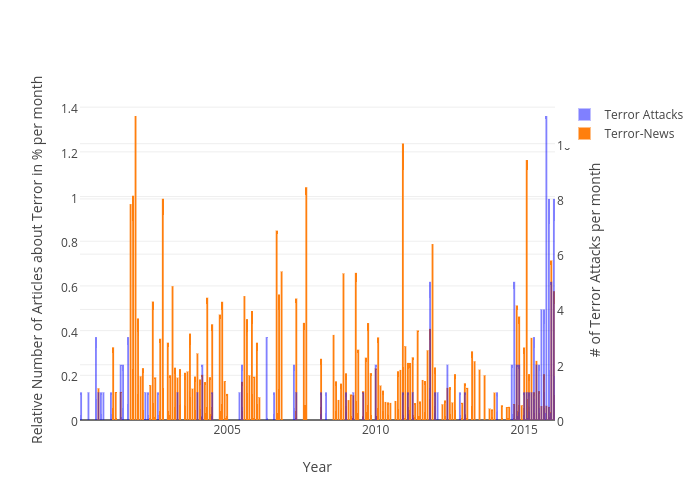
\includegraphics[width=.8\textwidth]{images/zeit/german_attacks}
    \caption{Terrorism-News and Number of Terrorism Attack (including Attempts)}
    \label{fig:zeit_terrorism_germany_attacks}
  \end{subfigure}
  \begin{subfigure}{1\textwidth}
    \centering
    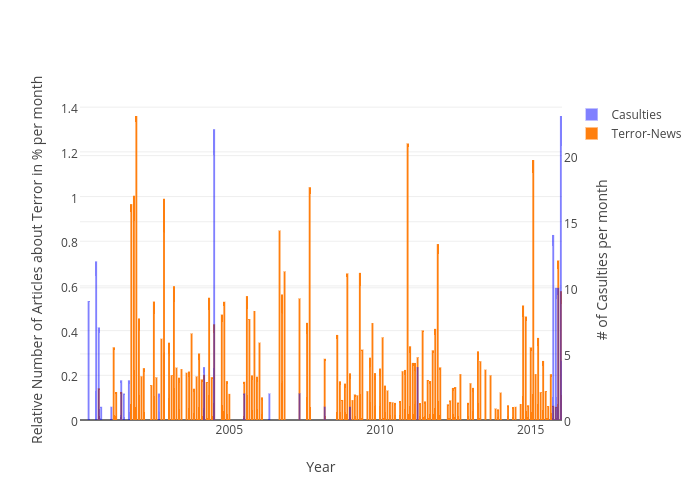
\includegraphics[width=.8\textwidth]{images/zeit/german_casulties}
    \caption{Terrorism-News and Number of Casulties (Injured + Killed)}
    \label{fig:zeit_terrorism_germany_casulties}
  \end{subfigure}
  \caption{Terrorism in Germany and News about Terrorism between 2000-2015}
  \label{fig:zeit_terrorism_germany}
\end{figure}
Both graphics in \autoref{fig:zeit_terrorism_germany} show, that the news in the Zeit doesn't correlate in a large scale.
While there are many terror-attacks (see \autoref{fig:zeit_terrorism_germany_attacks}) in the beginning of the century and even more at the end of 2015,
the Zeit published more news between end of 2001 to mid 2004 and between mid 2008 to end of 2011.
The first period of high frequency articles can be explained by the aftermath of 9/11 attacks,
dealing with, for example, security concerns that are related to Germany, too.

This shows that local news do not only report about terror when there are local incidents.
So we went further and also considered that local newspapers tend to cover not only local news,
but also news of their allies and reflect their situation onto themself.
Therefore we also included western countries in our research, i.e. countries in Western Europe and North America.
Similar to the filter-process to find articles related to Germany,
we used DBpedia to find out which countries are located in Western Europe and North America.
The process for GTD was very straight forward again,
as each recorded attack is also labeled with a region,
which include Western \textit{Europe} and \textit{North America}.

\begin{figure}[h]
  \centering
  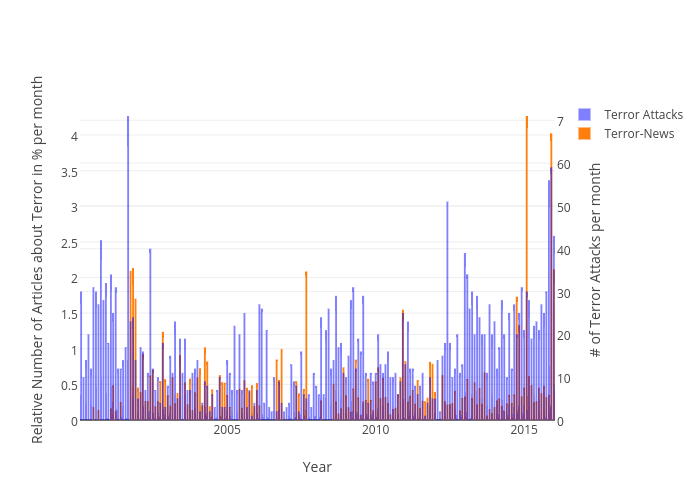
\includegraphics[width=.8\textwidth]{images/zeit/western_attacks}
  \caption{Terrorism-News and Number of Terrorism Attack (including Attempts)}
  \label{fig:zeit_terrorism_western_attacks}
\end{figure}
\autoref{fig:zeit_terrorism_western_attacks} shows the results of the above mentioned process.
Both datasets,
the number of terror attacks and the relative number of Articles about Terrorism,
are grouped into months again.
The two highes peaks with 4.2\% (January 2015) and 4\% (November 2015) of articles related to terrorism
are about the terror attacks in France (\textit{Charlie Hebdo shooting} respectively the \textit{Paris attacks})

\begin{figure}[h]
 \centering
 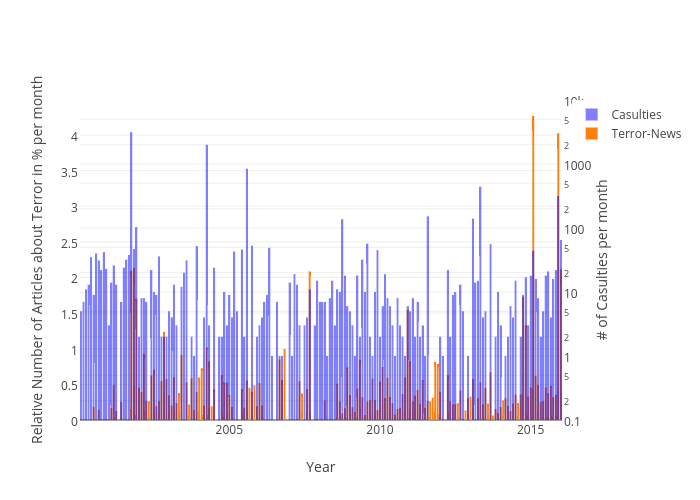
\includegraphics[width=.8\textwidth]{images/zeit/western_casulties}
 \caption{Terrorism-News and Number of Casulties (Injured + Killed)}
 \label{fig:zeit_terrorism_western_casulties}
\end{figure}
Here we look at the casulties instead of the number of attacks.
It is reasonable to believe that more articles about terrorism are published when the casulty-count reaches a certain threshold,
but higher casulties do not mean more more articles, we used a logarithmic scale for the number of casulties.


\input{4_discussion}
\input{5_conclusion}

% Acknowledgments here
\ACKNOWLEDGMENT{%
% Enter the text of acknowledgments here
}% Leave this (end of acknowledgment)


% Appendix here
% Options are (1) APPENDIX (with or without general title) or
%             (2) APPENDICES (if it has more than one unrelated sections)
% Outcomment the appropriate case if necessary
%
% \begin{APPENDIX}{<Title of the Appendix>}
% \end{APPENDIX}
%
%   or
%
% \begin{APPENDICES}
% \section{<Title of Section A>}
% \section{<Title of Section B>}
% etc
% \end{APPENDICES}


% References here (outcomment the appropriate case)

% CASE 1: BiBTeX used to constantly update the references
%   (while the paper is being written).
%\bibliographystyle{informs2014} % outcomment this and next line in Case 1
%\bibliography{<your bib file(s)>} % if more than one, comma separated

% CASE 2: BiBTeX used to generate mypaper.bbl (to be further fine tuned)
%\input{mypaper.bbl} % outcomment this line in Case 2

\end{document}
